\section{Trasformazione di Legendre vista più geometricamente}
\setcounter{equation}{0}

\begin{center}
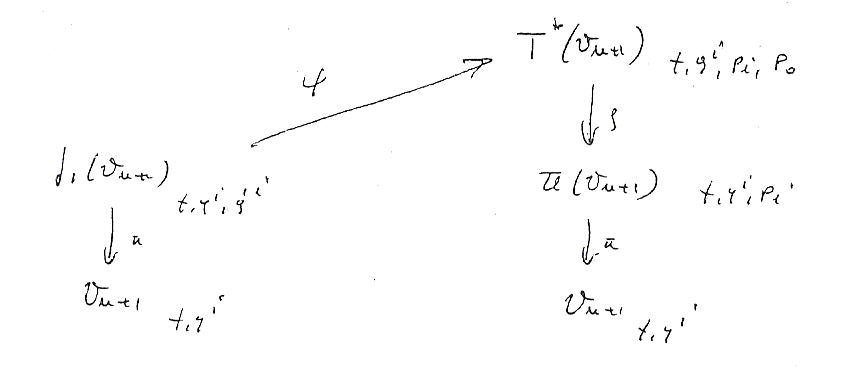
\includegraphics[width=\columnwidth]{media/trasformazione-di-legendre-vista-piu-geometricamente/26-1.jpg}
\end{center}

Vogliamo considerare una applicazione $ \psi : j_1 (\mathcal{V}_{n+1}) \longrightarrow T^* (\mathcal{V}_{n+1}) $. Dal punto di vista geometrico, essa vuole rappresentare una superficie di dimensione $ 2n+1 $ in $ T^* (\mathcal{V}_{n+1}) $, precisamente l'immagine $ \psi (j_1 (\mathcal{V}_{n+1})) $ in $ T^* (\mathcal{V}_{n+1}) $.

Richiediamo che $ \psi $ commuti con la proiezione $ \pi $, cioè preservi il punto in $ \mathcal{V}_{n+1} $. In coordinate, $ \psi $ sarà rappresentata nella forma
\begin{equation*}
\begin{split} 
	\psi : \quad &
\begin{cases}
	t = t \\
	q^i = q^i \\
	P_0 = P_0 (t, q^i, \dot{q}^i) \\
	P_i = P_i (t, q^i, \dot{q}^i) \\
\end{cases}
	\text{ ( $ \psi $ commuta con $ \pi $ ) }
\end{split}
\end{equation*}

Ricordiamo che, su $ j_1 (\mathcal{V}_{n+1}) $, (che, ricordiamo, rappresenta la totalità degli stati cinetici del sistema) dato un sistema dinamico Lagrangiano, abbiamo una funzione Lagrangiana $ \Lagr (t, q, \dot{q}) $ e una $ 1 $-forma di \textit{Poincaré-Cartan}
\begin{equation*}
	\theta_{\Lagr} = - H dt + \frac{\partial \Lagr}{\partial \dot{q}^i} dq^i \quad \qquad H = \frac{\partial \Lagr}{\partial \dot{q}^k} d\dot{q}^k - \Lagr
\end{equation*}

Su $ T^* (\mathcal{V}_{n+1}) $ abbiamo invece la $ 1 $-forma \textit{canonica di Liouville}
\begin{equation*}
	\theta = P_0 dt + P_i d \dot{q}^i
\end{equation*}

Sussiste il seguente risultato (trasformazione di Legendre): \\
Esiste un'unica $ \psi : j_1 (\mathcal{V}_{n+1}) \longrightarrow T^* (\mathcal{V}_{n+1}) $ fibrata in $ \mathcal{V}_{n+1} $ (cioè commutante con le proiezioni $ \pi :  j_1 (\mathcal{V}_{n+1}) \longrightarrow \mathcal{V}_{n+1} $  e $ \pi \cdot \rho : T^* (\mathcal{V}_{n+1}) \longrightarrow \mathcal{V}_{n+1} $ ) tale che
\begin{equation*}
	\theta_{\Lagr} = \psi^* (\theta)
\end{equation*}

In coordinate, questa condizione diventa
\begin{equation*}
\begin{cases}
	t = t \\
	q^i = q^i \\
	P_0 = - H (t, q^i, \dot{q}^i) \\
	P_i = \frac{\partial \Lagr}{\partial \dot{q}^i} (t, q^i, \dot{q}^i)
\end{cases}
	H = \frac{\partial \Lagr}{\partial \dot{q}^i} \dot{q}^i - \Lagr
\end{equation*}

\begin{center}
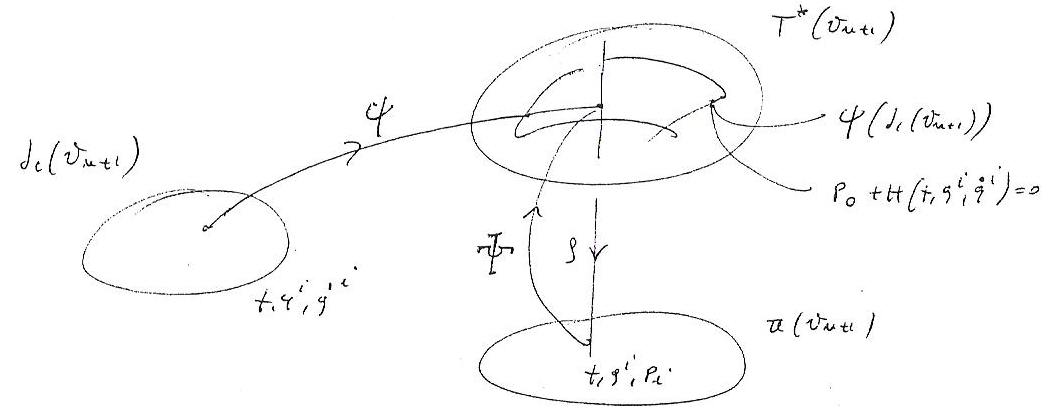
\includegraphics[width=\columnwidth]{media/trasformazione-di-legendre-vista-piu-geometricamente/26-2.jpg}
\end{center}

Ammesso, almeno localmente, che $ det \left( \frac{\partial^2 \Lagr}{\partial \dot{q}^i \partial \dot{q}^k} \right) \neq 0 $, la relazione $ P_i = \frac{\partial \Lagr}{\partial \dot{q}^i} (t, q^i, P_i) $ può essere posta nella forma
\begin{equation*}
	\dot{q}^i = \dot{q}^i (t, q^i, P_i)
\end{equation*}

e la funzione $ H $, definita inusualmente in funzione di $ t, q^i, \dot{q}^i $, può essere espressa in forma di $ t, q^i, P_i $:

% FINE PAGINA 26 - INIZIO PAGINA 27

\begin{equation*}
\begin{split}
H \left( t, q^i, P_i \right) &= \left( \frac{\partial \Lagr}{\partial \dot{q}^k} \dot{q}^k - \Lagr \right) \left( t, q^i, \dot{q}^i\left( t, q^i, P_i \right) \right) \\
&= \frac{\partial \Lagr}{\partial \dot{q}^k} \dot{q}^k \left( t, q^i, P_i \right) - \Lagr \left( t, q^i, \dot{q}^i\left( t, q^i, P_i \right) \right) \\
&= P_k \dot{q}^k \left( t, q^i, P_i \right) - \Lagr \left( t, q^i, \dot{q}^i \left( t, q^i, P_i \right) \right)
\end{split}
\end{equation*}

la superficie $ \Psi \left( j_1 (\mathcal{V}_{n + 1}) \right) $ può, a questo punto, essere espressa come luogo di zeri di

\begin{equation*}
P_0 + H \left( t, q^i, P_i \right) = 0
\end{equation*}

ovvero può essere rappresentata parametricamente nella forma

\begin{equation*}
t = t, \quad q^i = q^i, \quad P_i = P_i, \quad P_0 = - H \left( t, q^i, P_i \right)
\end{equation*}

come immagine attraverso $ \Psi $, di $ \pi(\mathcal{V}_{n + 1}) $.\\

La funzione $ H = H \left( t, q^i, P_i \right) $, riguardata come funzione di $ t, q^i, P_i $, è detta la \textit{funzione Hamiltoniana} del sistema (descritto dalla precedente Lagrangiana $ \Lagr $). \\

Con calcoli banali, abbiamo le ralazioni seguenti:

\begin{equation*}
\begin{split}
\frac{\partial H}{\partial P_r} = \dot{q}^r - \cancel{P_k \frac{\partial \dot{q}^k}{\partial P_r}} - \cancel{\frac{\partial \Lagr}{\partial \dot{q}^k} \frac{\partial \dot{q}^k}{\partial P_r}} = \dot{q}^r \\
\frac{\partial H}{\partial t} = \cancel{P_k \frac{\partial \dot{q}^k}{\partial t}} - \frac{\partial \Lagr}{\partial t} - \cancel{\frac{\partial \Lagr}{\partial t} \frac{\partial \dot{q}^k}{\partial t}} = - \frac{\partial \Lagr}{\partial t} \\
\frac{\partial H}{\partial q^i} = \cancel{P_k \frac{\partial \dot{q}^k}{\partial q^i}} - \frac{\partial \Lagr}{\partial q^i} - \cancel{\frac{\partial \Lagr}{\partial \dot{q}^k} \frac{\partial \dot{q}^k}{\partial q^i}} = - \frac{\partial \Lagr}{\partial q^i}
\end{split}
\end{equation*}

Infine, le equazioni di Lagrange

\begin{equation*}
\begin{cases}
\frac{dq^i}{dt} = \dot{q}^i \\
\frac{d}{dt} \frac{\partial \Lagr}{\partial \dot{q}^i} = \frac{\partial \Lagr}{\partial q^i}
\end{cases}
\end{equation*}

diventano, ponendo $ \frac{\partial \Lagr}{\partial \dot{q}^i} = P_i $

\begin{equation*}
\begin{cases}
\frac{dq^i}{dt} = \dot{q}^i \\
\frac{dP_i}{dt} = \frac{\partial \Lagr}{\partial q^i}
\end{cases}
\end{equation*}

e, per le relazioni dedotte sopra, %AAAAAAAAAAAAAAAAAAAAAAAAAAAAAAAAAAAAAAAAAA qui sarebbe utile inserire un ref

\begin{equation*}
\begin{cases}
\frac{dq^i}{dt} = \frac{\partial H}{\partial P_i} \\
\frac{dP_i}{dt} = - \frac{\partial H}{\partial q^i}
\end{cases}
\quad
H = H (t, q^i, P_i)
\end{equation*}

dette \textit{equazioni di Hamilton}, matematicamente equivalenti al campo

\begin{align*}
Z = \frac{\partial}{\partial t} + \frac{\partial H}{\partial P_i} \frac{\partial}{\partial q^i} - \frac{\partial H}{\partial q^i} \frac{\partial}{\partial P_i} \quad \text{ su } \pi(\mathcal{V}_{n + 1})
\end{align*}

Data una funzione $ f : \pi (\mathcal{V}_{n + 1}) \rightarrow \mathbb{R} $, $ f = f (t, q^i, P_i) $ l'evoluzione di $ f $ lungo i moti (cioè le curve in $ \pi(\mathcal{V}_{n + 1}) $ soluzioni delle equazioni di Hamilton) è data da

\begin{equation*}
\begin{split}
\frac{d}{d t} f &= \frac{\partial f}{\partial t} + \frac{\partial f}{\partial q^i} \frac{d q^i}{d t} + \frac{\partial f}{\partial P_i} \frac{d P_i}{d t} \\
&= \frac{\partial f}{\partial t} + \frac{\partial f}{\partial q^i} \frac{\partial H}{\partial P_i} - \frac{\partial f}{\partial P_i} \frac{\partial H}{\partial q^i} \\
&= \frac{\partial f}{\partial t} + \{ f, H \} \\
&= \{ f, P_0 \} + \{ f, H \}
\end{split}
\end{equation*}

% FINE PAGINA 27 - INIZIO PAGINA 28

con $ \{ f, H \} $ parentesi di Poisson in $ \pi(\mathcal{V}_{n + 1}) $ e $ \{ f, P_0 \} $ parentesi di Poisson in $ T^* (\mathcal{V}_{n+1}) $ (in $ \{ f, P_0 \} $, $ f $ viene riguardata ovviamente come funzione definita su $ T^* (\mathcal{V}_{n+1}) $, descitta ancora nella forma $ f = f (t, q^i, P_i) $). Riassumendo

\begin{equation*} \label{pag:trasf_leg_geom}
\frac{df}{dt} = \{ f, P_0 + H \} \qquad \qquad \longleftarrow \quad \text{parentesi di Poisson in $ T^* (\mathcal{V}_{n+1}) $}
\end{equation*}

In particolare, le equazioni di Hamilton diventano

\begin{equation*}
\begin{cases}
\frac{dq^i}{dt} = \{q^i, P_0 + H\} = \frac{\partial H}{\partial P_i} \\
\frac{dP_i}{dt} = \{P_i, P_0 + H\} = - \frac{\partial H}{\partial q^i}
\end{cases}
\end{equation*}

Infine

\begin{equation*}
\frac{dH}{dt} = \{H, P_0 + H\} = \{H, P_0\} = \frac{\partial H}{\partial t}
\end{equation*}

Facilmente si verificano i fatti seguenti:

\begin{itemize}
\item $ H $ non dipende esplicitamente dal tempo $ \Longrightarrow $ \, $ H $ integrale primo;
\item $ H $ non dipende esplicitamente da $ q^k $ $ \Longrightarrow $ \, $ P_k $ integrale primo;
\item $ f, g $ integrali primi $ \longrightarrow \{f, g\} $  integrale primo (conseguenza dell'identità di Jacobi).
\end{itemize}